\documentclass[a4paper,13.5pt]{extarticle}
\usepackage{geometry}
\usepackage[utf8]{inputenc}
\usepackage{amsmath,amssymb,graphicx,mathtools, nccmath, bigints}
\usepackage{caption,subcaption}
\usepackage{multirow}
\usepackage{float}
\usepackage{lipsum}
\usepackage{hyperref}
\usepackage{enumitem}
\usepackage[nodisplayskipstretch]{setspace}
\usepackage{booktabs}
\usepackage{mathtools}
\usepackage{etoolbox}
\usepackage{xcolor}
\usepackage[capitalize]{cleveref}
\usepackage{blindtext}
\usepackage{eso-pic,rotating,graphicx}
\usepackage{microtype}
\usepackage{scalerel}


\newcommand{\argmax}{\operatornamewithlimits{argmax}}
\def\am{$\theta_{\scaleto{\text{AM}}{2pt}}$}
\title{WFST enabled Minimum Bayes Risk~(MBR) Training}
\author{Tina Raissi}

\begin{document}
	
	\maketitle
	
	\section{Training Criterion}
	For an acoustic feature sequence $X = x_1^T$ and a word sequence $W = w_1^N$, of length $T$ and $N$, respectively, define the output sequence $a_1^S$ corresponding to $W$.\  This can be phonemes, wordpieces, or characters.
	
	For a set of parameters $\theta$, the statistical formulation of automatic speech recognition task based on maximum a-posteriori probability~(MAP) calculates the Bayes risk via a loss function $L(.,.)$ as follows 
	
	\begin{align}
		\label{BayesRisk}
		\mathcal{R_{\text{B}}}(\theta) = \sum_{\bar{W} \in \mathcal{W}} \sum_{W\in \mathcal{W}} \bigintssss p_{_\theta}(W | X) L(\bar{W}, W)  pr(\bar{W} , X)dX
	\end{align}
	where $\mathcal{W}$ is the hypothesis space, and $\bar{W}$ is the correct hypothesis for $X$.  Note the following points:
	
	\begin{itemize}
		\item Not every loss function is suitable in terms of a tractable computation. We need a loss that considers local dependency, e.g., Hamming distance.
		\item if $L$ is Levenshtein distance, then \cref{BayesRisk} gives the expected word error rate~(WER)
		\item The true probability distribution $ pr(\bar{W} , X)$ is generally not known, in practice we approximate this with a given training data
	\end{itemize}
	
	For a finite training set of utterances $\{X\}_{r=1}^M$, we define an accuracy function $A(.,.)$. The training in \cref{BayesRisk2} is known as \textit{minimum Bayes risk}\cite{gibson2006hypothesis}
	
	\begin{align}
		\label{BayesRisk2}
		\mathcal{F_{\text{BR}}}(\theta) = \frac{1}{M}\sum_{r=1}^M\sum_{W \in \mathcal{W}} p_{_\theta}(W | X^r) A(\bar{W^r}, W)
	\end{align}
	
	
	It is possible to have different accuracy functions on phone or state level for minimum phone error~(MPE)\cite{povey2002minimum} and state-level minimum Bayes risk~(sMBR) trainings, respectively.\ By using log probabilities and accuracy function equal to Kronecker delta we end up in maximum mutual information~(MMI) training.
	It is possible to reformulate \cref{BayesRisk2} via the Bayes identity as: 
	
	\begin{align}
		\label{BayesRisk3}
		\mathcal{F_{\text{BR}}}(\theta) = \sum_{r=1}^M\sum_{W \in \mathcal{W}} \frac{p_{_{\theta_{\scaleto{\text{AM}}{2pt}}}}(X^r | W)p_{_{\theta_{\scaleto{\text{LM}}{2pt}}}}(W)  A(\bar{W^r}, W)}{\sum_{W^{\prime}} p_{_{\theta_{\scaleto{\text{AM}}{2pt}}}}(X^r | W^{\prime})p_{_{\theta_{\scaleto{\text{LM}}{2pt}}}}(W^{\prime})}
	\end{align}
	
	where $\theta=\{\theta_{\scaleto{\text{AM}}{2pt}}, \theta_{\scaleto{\text{LM}}{2pt}}\}$, consisting of acoustic and language model parameters. Assume we are already given an LM. 
	
	\section{WFST/Graph Representation}
	
	For decoding or sequence discriminative training we generally need to consider the set of all possible word sequences called also as the hypothesis space. This can be done by taking an N-best list of the most likely hypotheses or to use lattices, called sometimes also as graphs or Lattices.
	
	A transducer $\mathcal{L}$ is an a-cyclic graph where nodes represent the time steps and edges represent the words. Each arc can be augmented with weights. Each path $\pi$ through $\mathcal{L}$  consists of a sequence of edges $e_1^N$ corresponding to a word sequence of length $N$. \ The edges carry the product of the acoustic and language model.
	
	\begin{align}
		\label{probpath}
		p(e_1^N, X) = \prod_{n=1}^N w[e_n]
	\end{align}
	
	The probability of a certain word within the sequence is equal to the sum over probability of all transducer paths $\pi(\mathcal{L})$ going through that specific edge:
	
	\begin{align}
		\label{probedge}
		p(e | X) = \sum_{\substack{e_1^N \in \pi(\mathcal{L})\\ \exists n: e_n=e}}p(e_1^N | X)
	\end{align}
	
	The sum over all paths is generally carried out via forward-backward algorithm.\footnote{For notation completeness refer also to Lucas' document}. Denote forward and backward scores accumulated at a certain transducer node $s$ by $\phi(s)$ and $\psi(s)$, respectively. For partial edge sequences $e_1^k$ and  $e_h^N$ reaching the edge $e$ in forward and backward paths we have
	
	\begin{align}
		\label{fwdbkwd}
		\mathbf{fb}(e, X)  = \sum_{\substack{e_1^k: \\ n[e_k] = p[e]}}\prod_{m=1}^k w[e_m] \cdot w[e] \cdot  \sum_{\substack{e_h^N: \\ p[e_h] = n[e]}}\prod_{n=h}^N w[e_n] 
	\end{align}
	
	Following \cref{fwdbkwd}, we can calculate the prior as $\phi(F) = p(X)$. Consequently, it is possible to calculate the arc posterior as $\mathbf{fb}(e | X) = \frac{	\mathbf{fb}(e, X)}{ p(X)}$.
	
	\section{Expectation Semiring}
	
	It is possible to define a specific semiring for the operations on the transducer. Typically, the MBR training relies on the \textit{expectation semiring}\cite{eisner2001expectation} defined with the following operations:
	
	\begin{itemize}
		\item  Each edge is augmented with the weight $(p,v) \in \mathbb{R}^+\times\mathbb{R}$ of probability and value
		\item $ (p_1,v_1)\oplus (p_2,v_2) = (p_1+p_2,v_1+v_2)$
		\item $ (p_1,v_1)\otimes (p_2,v_2)  = (p_1p_2, p_1v_2 + v_1p_2)$
		\item $\bar{1} = (1,0)$
		\item $\bar{0} = (0,0)$
		\item $inv(p,v) = (p^{-1}, - p^{-2}v)$
	\end{itemize} 
	
	
	
	
	\begin{figure}[t]
		\centering
		\caption*{Definition of different semirings relevant for training and decoding in ASR.(Source: \cite{hoffmeister2011wfst})}
		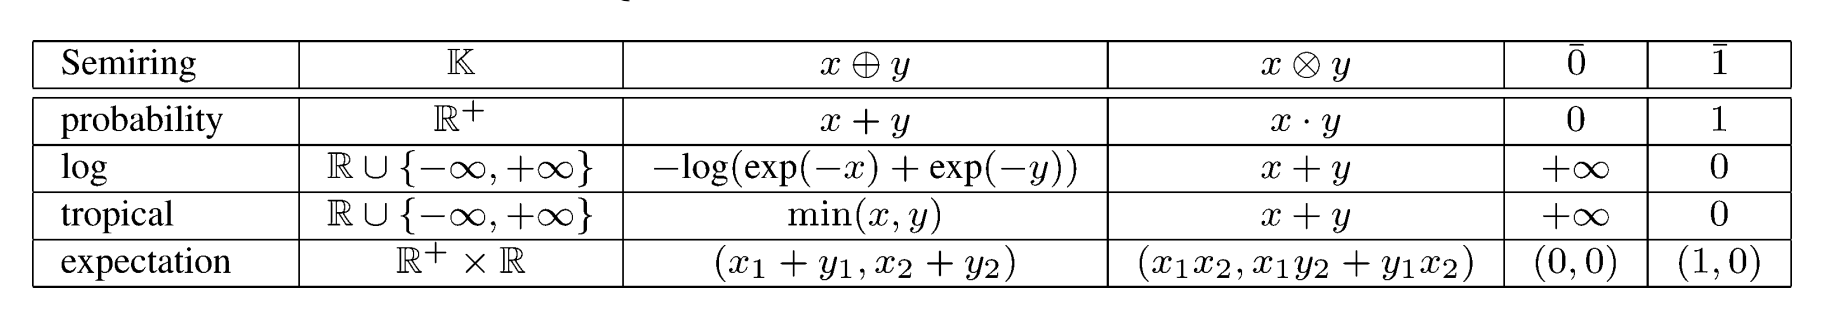
\includegraphics[width=1.\linewidth]{figures/semirings}	
	\end{figure}
	
	
	We augment each arc of the transducer with the pair $(p, v)$, where $p$ is similar to the arc weights when we have a probability semiring, i.e. $w[e][p] = p$. For a certain cost $c$, e.g. the value of the accuracy function, the value is initialized as $w[e][v] = w[e][p] \cdot c[e]$. The cost shall be additive along each path in the transducer:
	
	\begin{align}
		\label{addcost}
		c(e_1^N) = \sum_{n=1}^N c[e_n]
	\end{align}
	
	The forward-backward computation on the transducer using the expectation semiring makes use of the accumulated forward and backward scores at a certain node $s$, as shown in \cref{fwd} and \cref{bwd}, respectively. 
	
	
	\begin{align}
		\label{fwd}
		\phi(s)= \bigoplus_{\substack{e_1^n: \\ n[e_n]=s}} \bigotimes_{m=1}^n w[e_m]
	\end{align}
	
	
	\begin{align}
		\label{bwd}
		\psi(s)= \bigoplus_{\substack{e_1^n: \\ p[e_n]=s}} \bigotimes_{m=1}^n w[e_m]
	\end{align}
	
	The multiplication of the weights of the arcs through the transducer in the above equations can be roken down into the multiplication of the probabilities over a transducer using the probability semiring, and the cross multiplication between cost and probability for the value as follows:
	
	
	
	\begin{align}
		\label{prod}
		\bigotimes_{n=1}^N w[e_n] =  \bigotimes_{n=1}^N (p_n, v_n) = \left(\prod_{n=1}^N p_n,  \sum_{n=1}^N v_n \prod_{\substack{m=1 \\ m \neq n}} p_m\right)
	\end{align}
	
	You can see the first element of the resulting tuple in \cref{prod} as a probability distribution over the paths in the transducer, since the sum over all paths of this would sum up to one.\ The second element would represent the expected cost.\ We show this in relation to the sMBR gradient in \cref{smbr}.\ For the calculation of the expected cost we use the probability and the value components of the forward-backward values with the interpretations shown in \cref{fbp} and \cref{fbv}, respectively.
	
	\begin{align}
		\label{fbp}
		\mathbf{fb}(e, X)[p] = p(e, X)
	\end{align}
	
	\begin{align}
		\label{fbv}
		\mathbf{fb}(e, X)[v] = p(e, X)\cdot c[e]
	\end{align}
	
	By using \cref{fbp,fbv} this would be equivalent to we can calculate the cost of each arc as:
	
	\begin{align}
		\label{ce}
		c[e] = \frac{\mathbf{fb}(e, X)[v]}{\mathbf{fb}(e, X)[p]}
	\end{align}
	
	
	\section{Gradient of MBR Training Criterion}
	
	We calculate the derivative $\frac{\partial\mathcal{F_{\text{BR}}}}{\partial \theta_{\scaleto{\text{AM}}{2pt}}}$ with respect only to the acoustic model parameters.\ For simplicity, we define the expected cost for $r$-th utterance under the choice of \am and the loss function as shown in \cref{EA}.
	\begin{align}
		\label{EA}
		\mathbb{E}_{p_\text{\am}}[A_r]= \sum_W \frac{p_{_{\theta_{\scaleto{\text{AM}}{2pt}}}}(X^r | W)p_{_{\theta_{\scaleto{\text{LM}}{2pt}}}}(W)  A(\bar{W^r}, W)}{\sum_{W^{\prime}} p_{_{\theta_{\scaleto{\text{AM}}{2pt}}}}(X^r | W^{\prime})p_{_{\theta_{\scaleto{\text{LM}}{2pt}}}}(W^{\prime})}
	\end{align}
	
	In the following steps, we denote ${s_1^{T_r}}$ as the aligned hidden state sequence to the utterance $X^r$. The relation between the state sequence and the word sequence is defined by an intermediate mapping step, where we assign one output label to each state.\ In standard Hybrid NN/HMM this can be a generalized triphone (CART label). One can define any type of state-tying. We assume there is a unique mapping of the output label to a certain word sequence.\ Given this two deterministic and unique mapping steps, we can drop the dependency to the word sequence and operate on the state level.
	
	Similarly to maximum likelihood criterion~(ML) criterion, the derivative can be seen as the sum over the training utterances and over time of weighted log derivatives. The weights are normalized state occupancies and state accuracies in ML and MBR, respectively. By using the definition of state accuracy $a(s|X^r)$ in \cref{sl}, we have the derivative of \cref{derivative}, as shown in \cite{hoffmeister2011wfst}.
	
	
	
	\begin{align}
		\label{sl}
		a(s|X^r)=  \sum_W  \left[ \left( A(\bar{W^r}, W) - \mathbb{E}_{p_\text{\am}}[A_r] \right) \cdot\sum_{s_1^{T_r}|W: s_t=s} \frac{p_{_{\theta_{\scaleto{\text{AM}}{2pt}}}}(X^r , s_1^{T_r})p(W)}{\sum_{W^{\prime}} p_{_{\theta_{\scaleto{\text{AM}}{2pt}}}}(X^r , W^{\prime})} \right]
	\end{align}
	
	
	\begin{align}
		\label{derivative}
		\frac{\partial\mathcal{F_{\text{BR}}}}{\partial \theta_{\scaleto{\text{AM}}{2pt}}} =   \sum_{r=1}^M \mathbb{E}_{p_\text{\am}}[A_r]  \sum_{t=1}^{T_r} a(s|X^r) \frac{\partial \log  p_{_{\theta_{\scaleto{\text{AM}}{2pt}}}}(x_{rt}|s_t)}{\partial \theta_{\scaleto{\text{AM}}{2pt}}}
	\end{align}
	
	\newpage
	\section{SMBR  Training with Semiring Operations}
	\label{smbr}
	
	It is possible to express the derivative in terms of semiring operations.\ We need the following points:
	\begin{itemize}
		\item $\mathbf{P}$ : a probability WFST on state level, where each arc has the information about the time step and the state, with $w[e] = p_{_{\theta_{\scaleto{\text{AM}}{2pt}}}}(x_{t}, s_t | .)$.
		\item  $\mathbf{A}$ :  an accuracy WFST with the same structure as $\mathbf{P}$ but with arc weights having the value from the $A(.,.)$
		\item  $\mathbf{E}$ : an auxiliary WFST with the same structure as $\mathbf{P}$ and $\mathbf{A}$ with arc weights $w_{\mathbf{E}}[e] := (w_{\mathbf{P}}[e], w_{\mathbf{P}}[e]w_{\mathbf{A}}[e])$
		\item  $\mathbf{Q}$: an expectation WFST that has posterior probabilities from $\mathbf{P}$  as the first element and expected accuracy of the arc
		\item $\nabla \log \mathbf{P}$:  gradient WFST that has the derivative of the $\log$ probabilities from $\mathbf{P}$
		\item Formulation of the expected cost in terms of forward-backward scores in expectation semiring
		
	\end{itemize}
	
	The expected cost is defined as the sum over expected cost of the arcs and can be shown as follows:
	
	\begin{align*}
		\mathbb{E}_{p_\text{\am}}[\mathbf{A}_r] &= \frac{\sum_{e_1^N} w_{\mathbf{E}}[e_1^N][p] \cdot w_{\mathbf{E}}[e_1^N][c]}{p(X)}\\
		&=	\sum_{e_1^N} p(e_1^N|X)c(e_1^N)\\
		&=	\sum_{e} p(e|X)c(e)
	\end{align*}
	
	
	In practice this is done by taking the probability and value components of a complete forward pass. 
	
	\begin{align}
		\label{c}
		\mathbb{E}_{p_\text{\am}}[\mathbf{A}_r] = \frac{\phi(F)[v]}{\phi(F)[p]}
	\end{align}
	
	It has been shown that the gradient in \cref{derivative} can be written via semiring computation\cite{heigold2008modified}.\ Namely, by using the covariance of the gradient WFST $\nabla \log \mathbf{P}$ and $\mathbf{A}$ with respect to $\mathbf{P}$. This will lead to \cref{gradient} with the definition in \cref{cov}.\
	
	\begin{align}
		\label{gradient}
		\nabla \mathcal{F_{\text{BR}}} =   \sum_{r=1}^M \mathbb{E}_{p_\text{\am}}[A_r] \mathbf{Cov}(\mathbf{A}_r, \nabla \log \mathbf{P}_r)
	\end{align}
	
	
	
	\begin{align}
		\label{cov}
		\mathbf{Cov}(\mathbf{A},  \nabla \log \mathbf{P}) = \sum_{e \in \mathbf{P}} w_{\mathbf{Q}}[e][v]. w_{\mathbf{\nabla \log P}}[e]
	\end{align}
	
	
	
	
	\bibliographystyle{IEEEtran}
	\bibliography{mybib}
	
	
	
	
	
	
	
	
	
	
\end{document}
